\pagebreak
\section{Badania}
  W celu zbadania działania algorytmu MCTS został przeprowadzony eksperyment, w którym gracz 
  oparty o algorytm MCTS prowadził rozgrywki z agentami zachłannymi (opisanymi w poprzednim 
  rozdziale). Ze względu na duży czynnik losowości w grze, dla każdej pary (MCTS, agent) zostało
  rozegranych 100 gier, przy czym w połowie gracz MCTS zaczynał rozgrywkę, a w reszcie agent.
  W ramach każdej rozgrywki zostały obliczone następujące parametry:
  \begin{itemize}
    \item{całkowity czas rozgrywki,}
    \item{liczba przeprowadzonych symulacji,}
    \item{średni procent odwiedzonych dzieci węzła,}
    \item{maksymalna głębokość liścia,}
    \item{średnia głębokość liścia,}
    \item{mediana głębokości liści.}
  \end{itemize}

  Opracowane wyniki badań zostały przedstawione poniżej. Pionowe linie na wykresach wyznaczają
  granicę między kolejnymi turami gracza MCTS. W przypadku rozgrywek z agentem losowym, limit 
  czasowy działania algorytmu MCTS został ustalony na 30 sekund, natomiast dla pozostałych agentów
  (agresywny, kontrolujący) na 60 sekund.

  \begin{table}[H]
          \centering
          \begin{tabular}{|c|c|c|c|c|c|}
                  \hline
                  \multirow{2}{*}{\textbf{Gracz 1}} & \multirow{2}{*}{\textbf{Gracz 2}} & \multicolumn{2}{|c|}{\textbf{Wygrane}} & \multicolumn{2}{|c|}{\textbf{Przegrane}} \\
                  \cline{3-6}
                  & & \textbf{\%} & \textbf{Czas [s]} & \textbf{\%} & \textbf{Czas [s]} \\
                  \hline
                  Agresywny & MCTS & 0 & -- & 100 & 481 \\
                  \hline
                  MCTS & Agresywny & 10 & 541 & 90 & 300  \\
                  \hline \hline
                  Kontrolujący & MCTS & 100 & 780 & 0 & --  \\
                  \hline
                  MCTS & Kontrolujący & 80 & 663 & 20 & 720 \\
                  \hline \hline
                  Losowy & MCTS & 50 & 393 & 50 & 434 \\
                  \hline
                  MCTS & Losowy & 70 & 120 & 30 & 393 \\ 
                  \hline
          \end{tabular}
          \caption{Zestawienie wyników badań.}
  \end{table}

  \pagebreak
  \subsection{MCTS i agent losowy}

    \begin{figure}[H]
        \center
        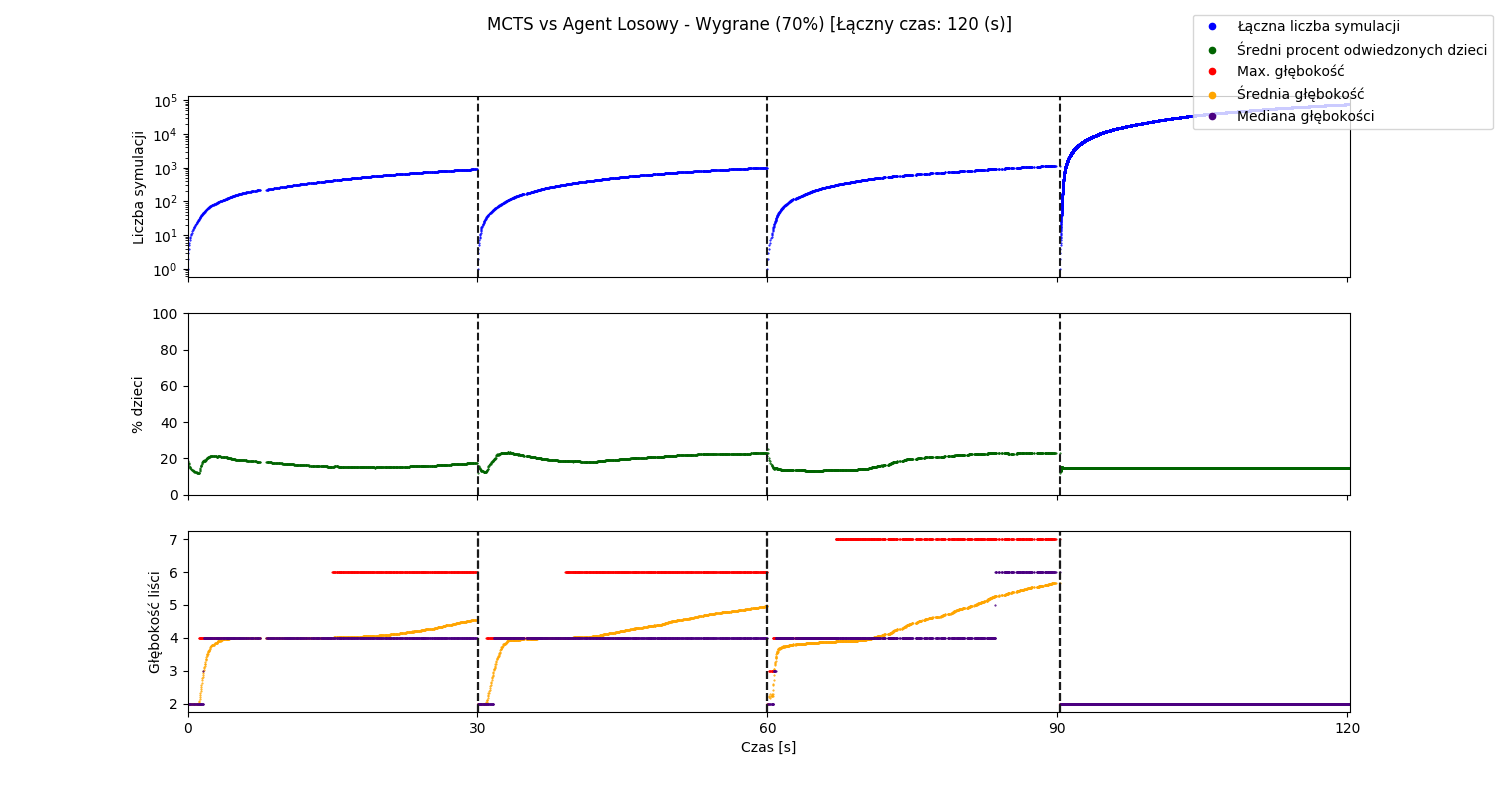
\includegraphics[width=\textwidth]{imgs/plots/MCTS_RA_WIN.png}
    \end{figure}

    \begin{figure}[H]
        \center
        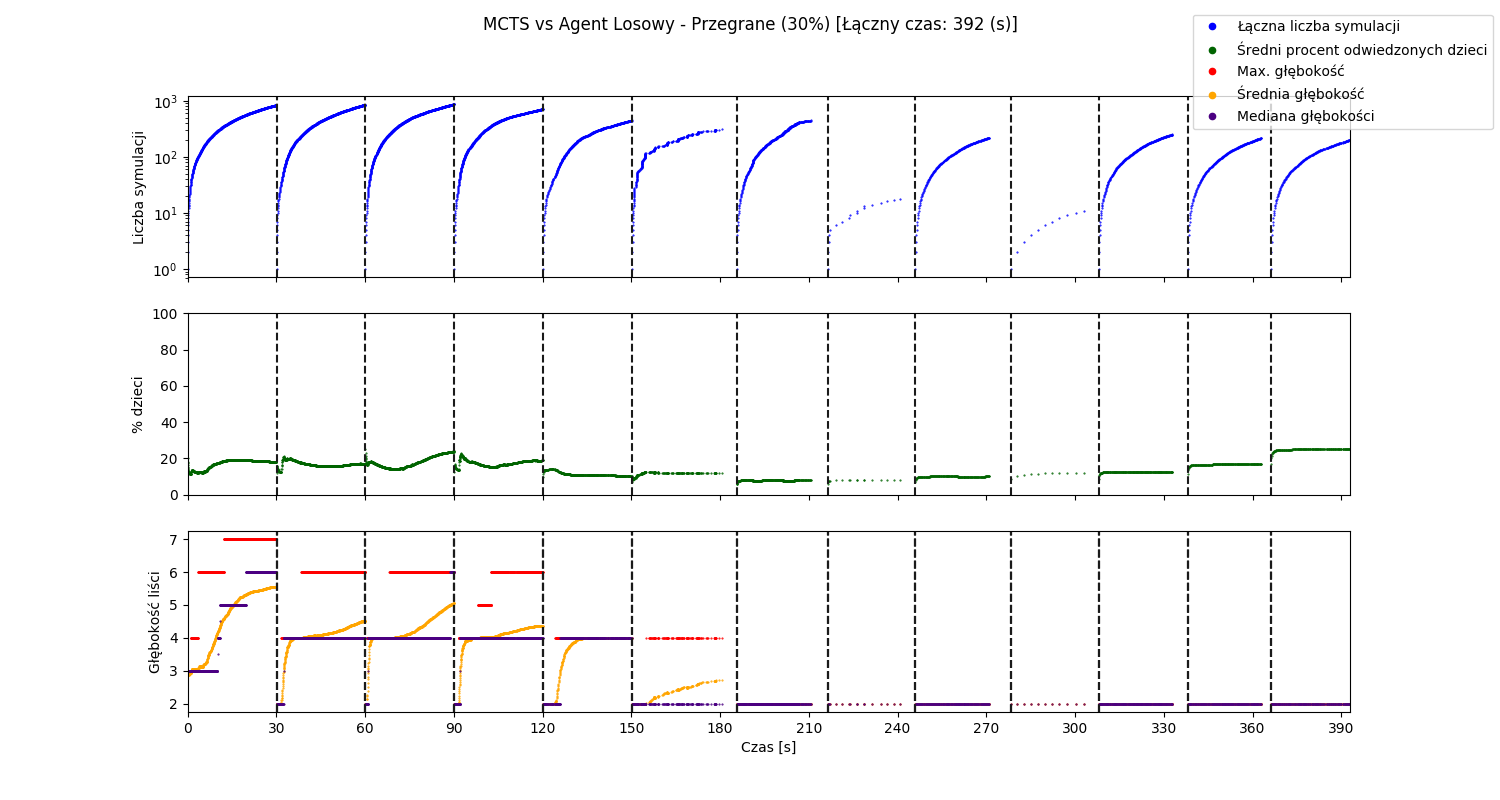
\includegraphics[width=\textwidth]{imgs/plots/MCTS_RA_LOST.png}
    \end{figure}

    \begin{figure}[H]
        \center
        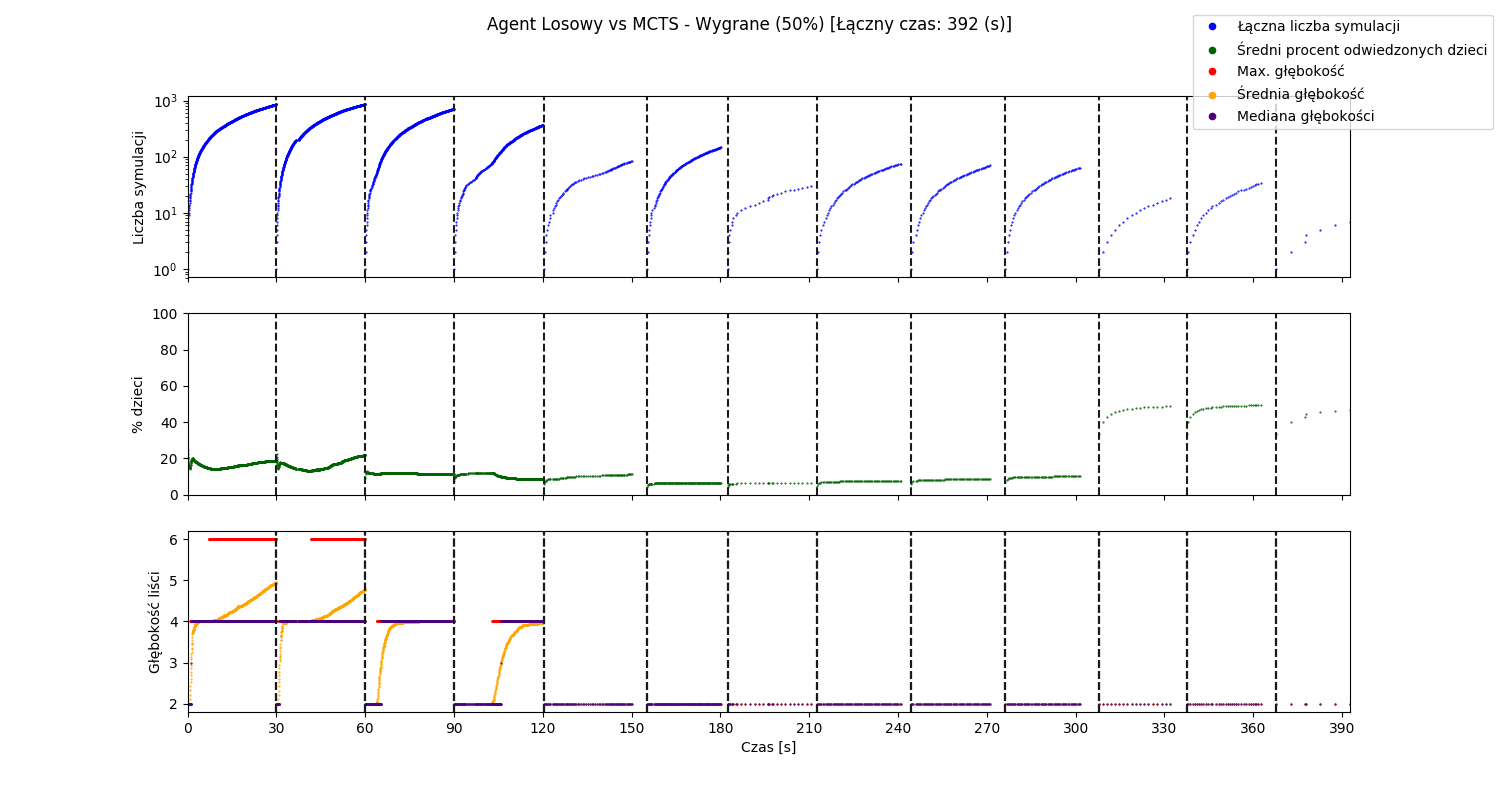
\includegraphics[width=\textwidth]{imgs/plots/RA_MCTS_WIN.png}
    \end{figure}

    \begin{figure}[H]
        \center
        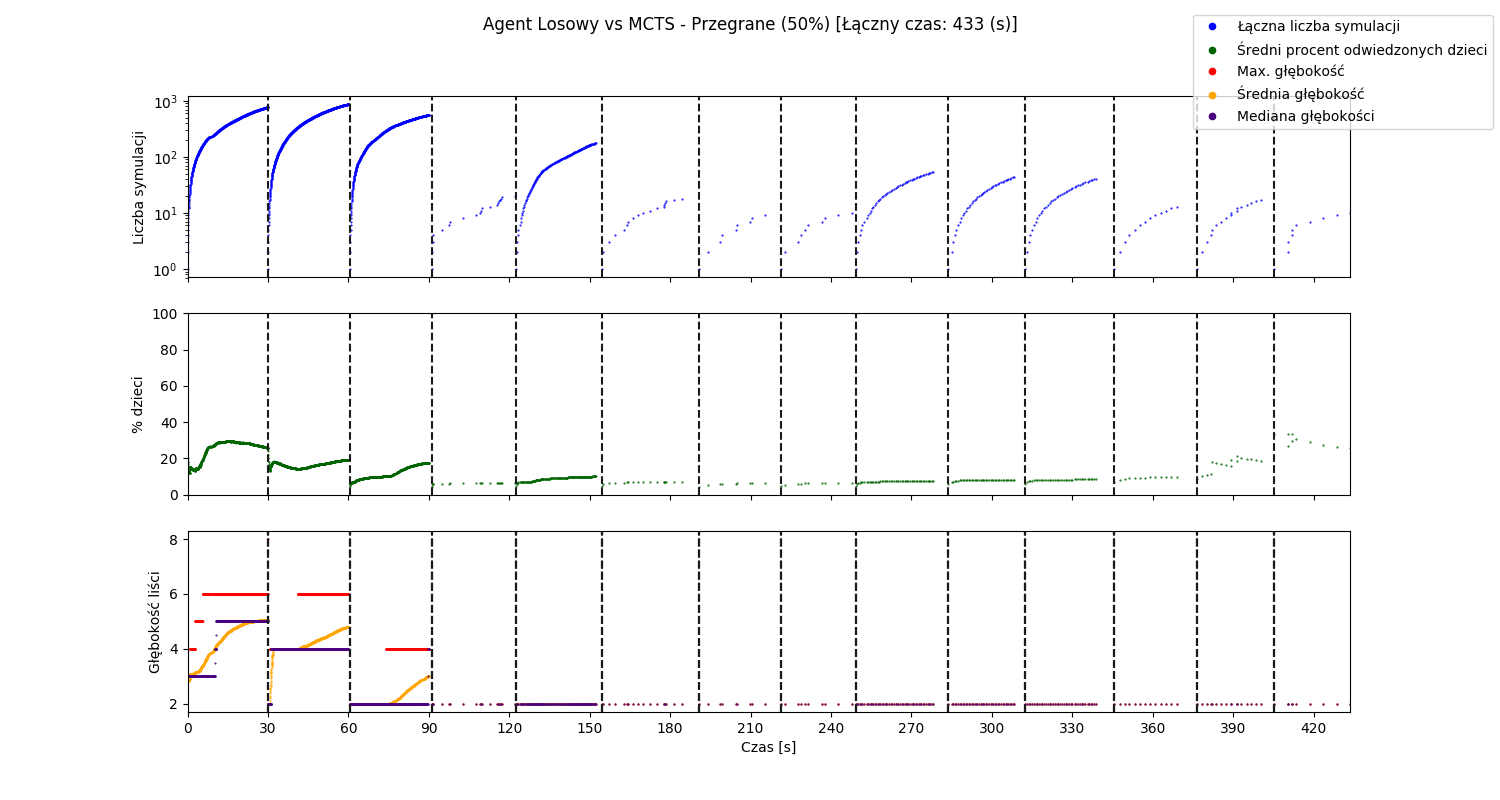
\includegraphics[width=\textwidth]{imgs/plots/RA_MCTS_LOST.png}
    \end{figure}


  \pagebreak
  \subsection{MCTS i agent agresywny}

    \begin{figure}[H]
        \center
        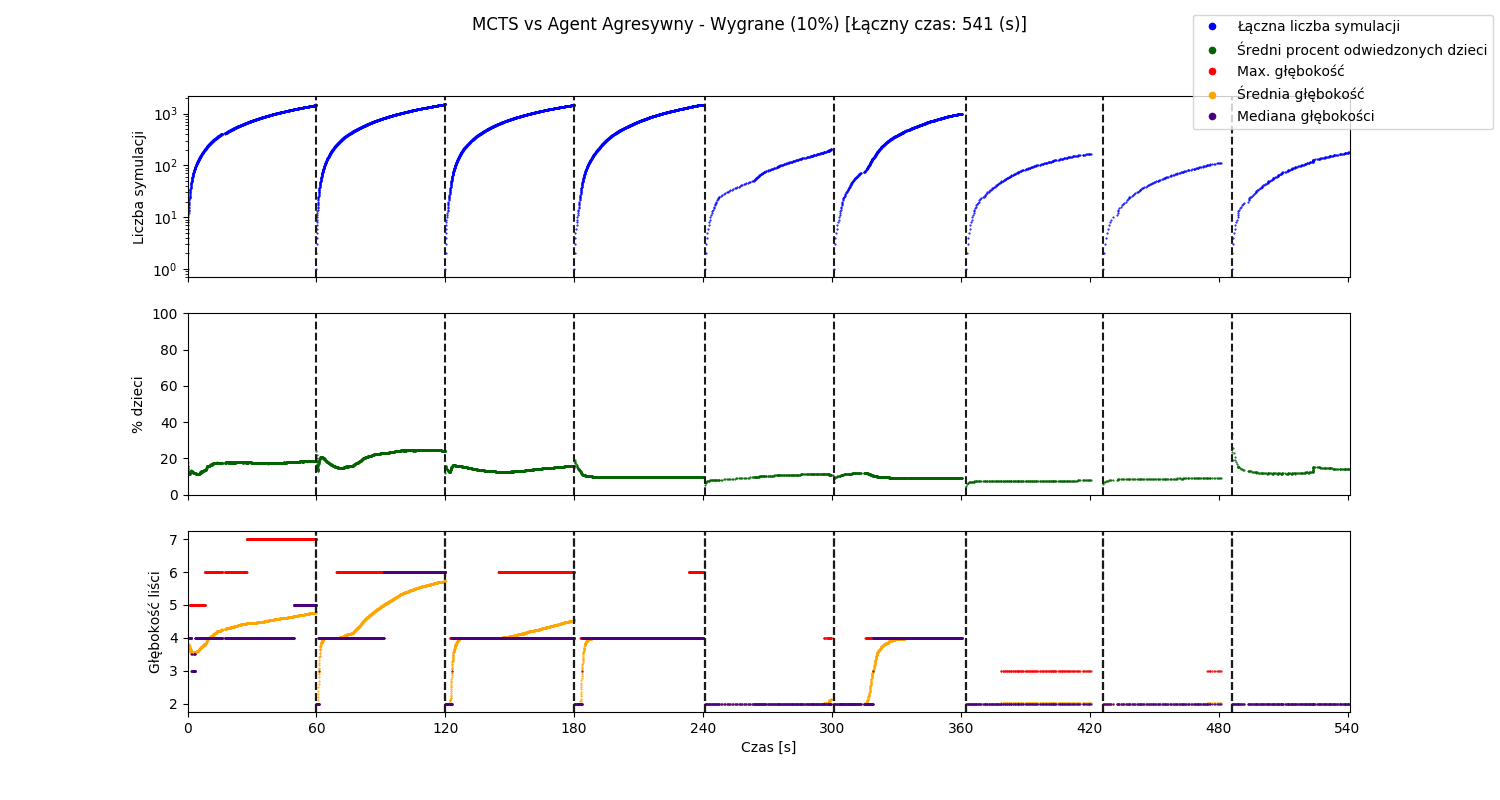
\includegraphics[width=\textwidth]{imgs/plots/MCTS_AA_WIN.png}
    \end{figure}

    \begin{figure}[H]
        \center
        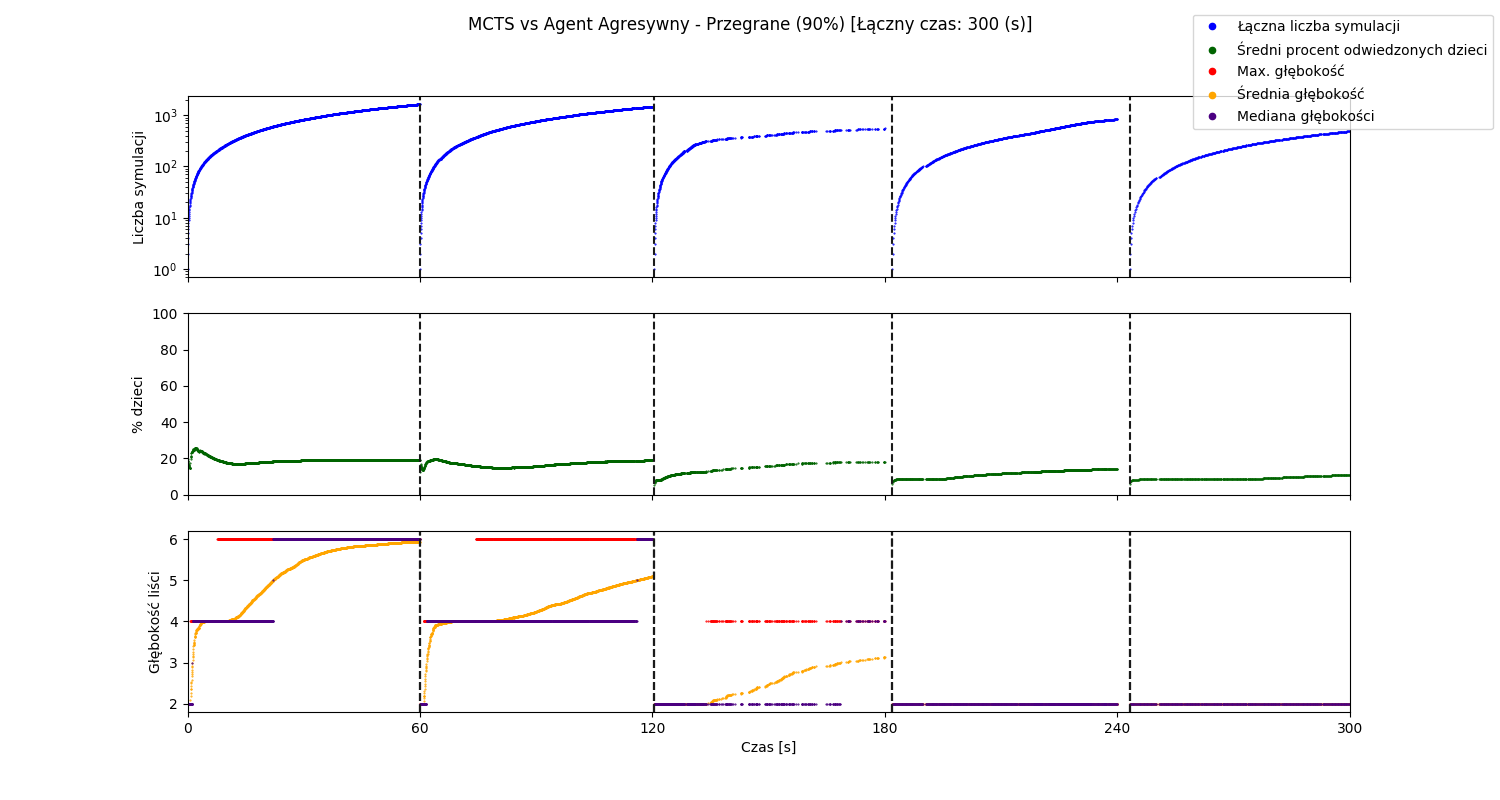
\includegraphics[width=\textwidth]{imgs/plots/MCTS_AA_LOST.png}
    \end{figure}

    \begin{figure}[H]
      \center
      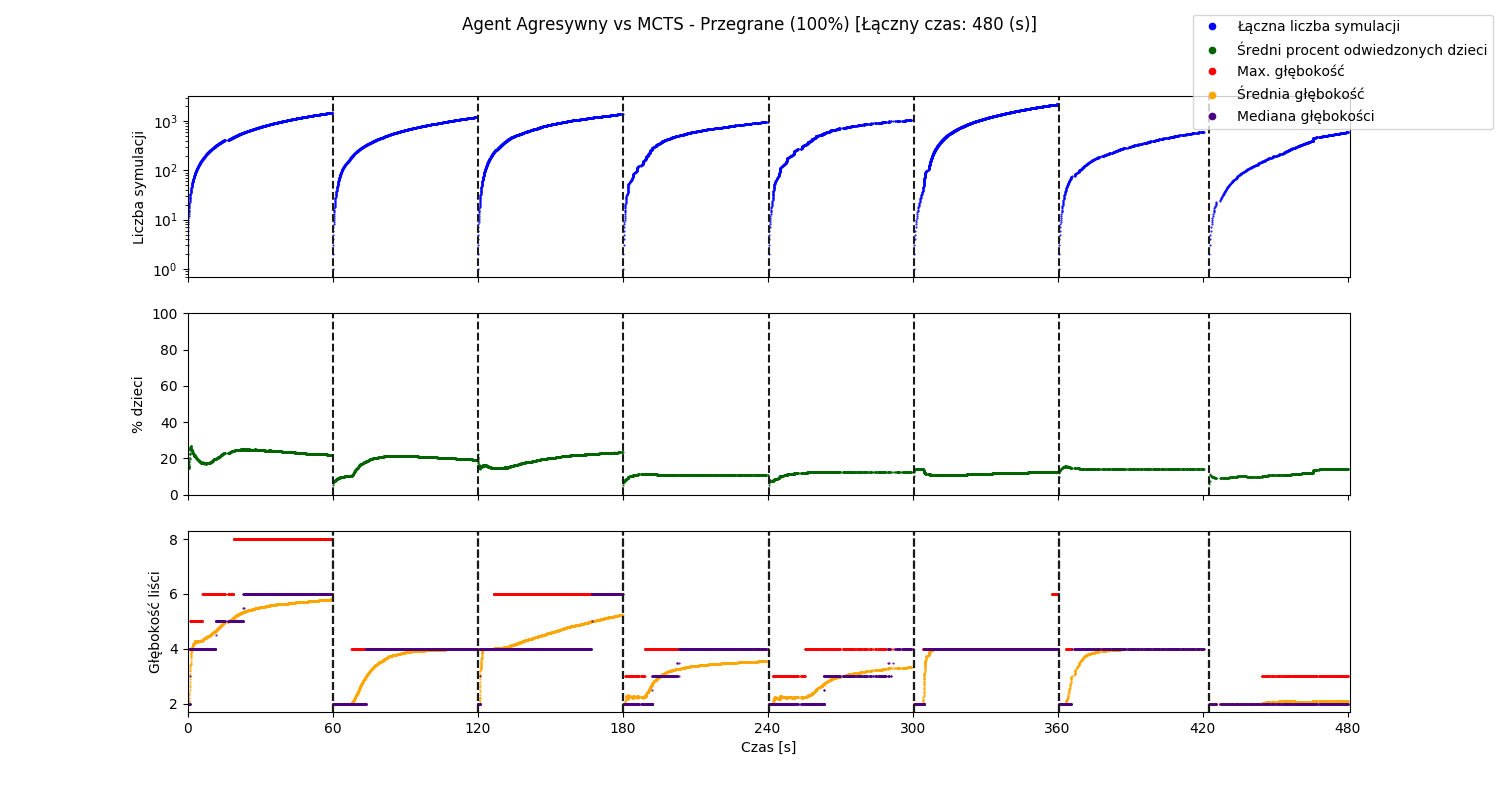
\includegraphics[width=\textwidth]{imgs/plots/AA_MCTS_LOST.png}
    \end{figure}


  \pagebreak
  \subsection{MCTS i agent kontrolujący}

    \begin{figure}[H]
        \center
        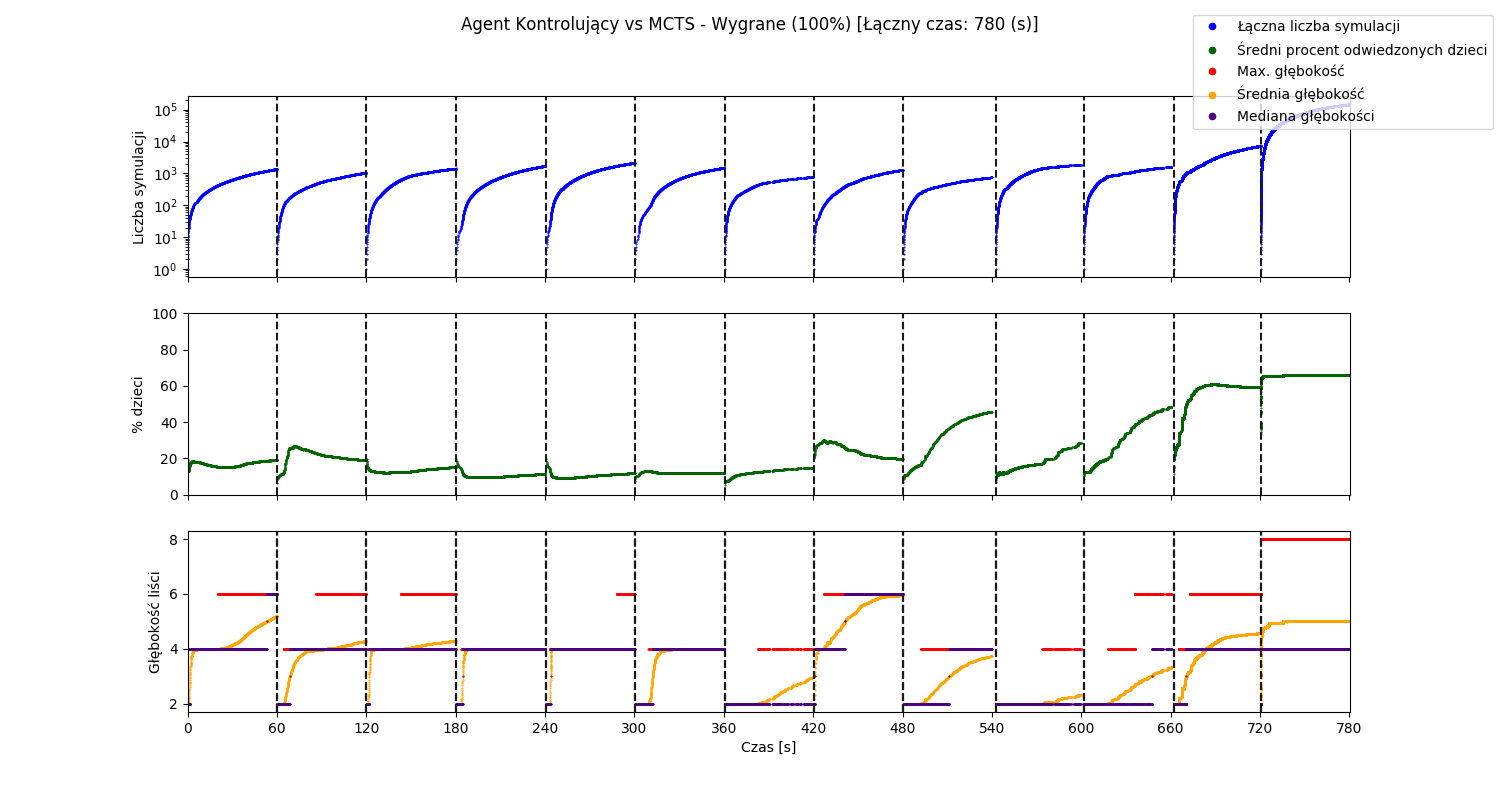
\includegraphics[width=\textwidth]{imgs/plots/CA_MCTS_WIN.png}
    \end{figure}

    \begin{figure}[H]
        \center
        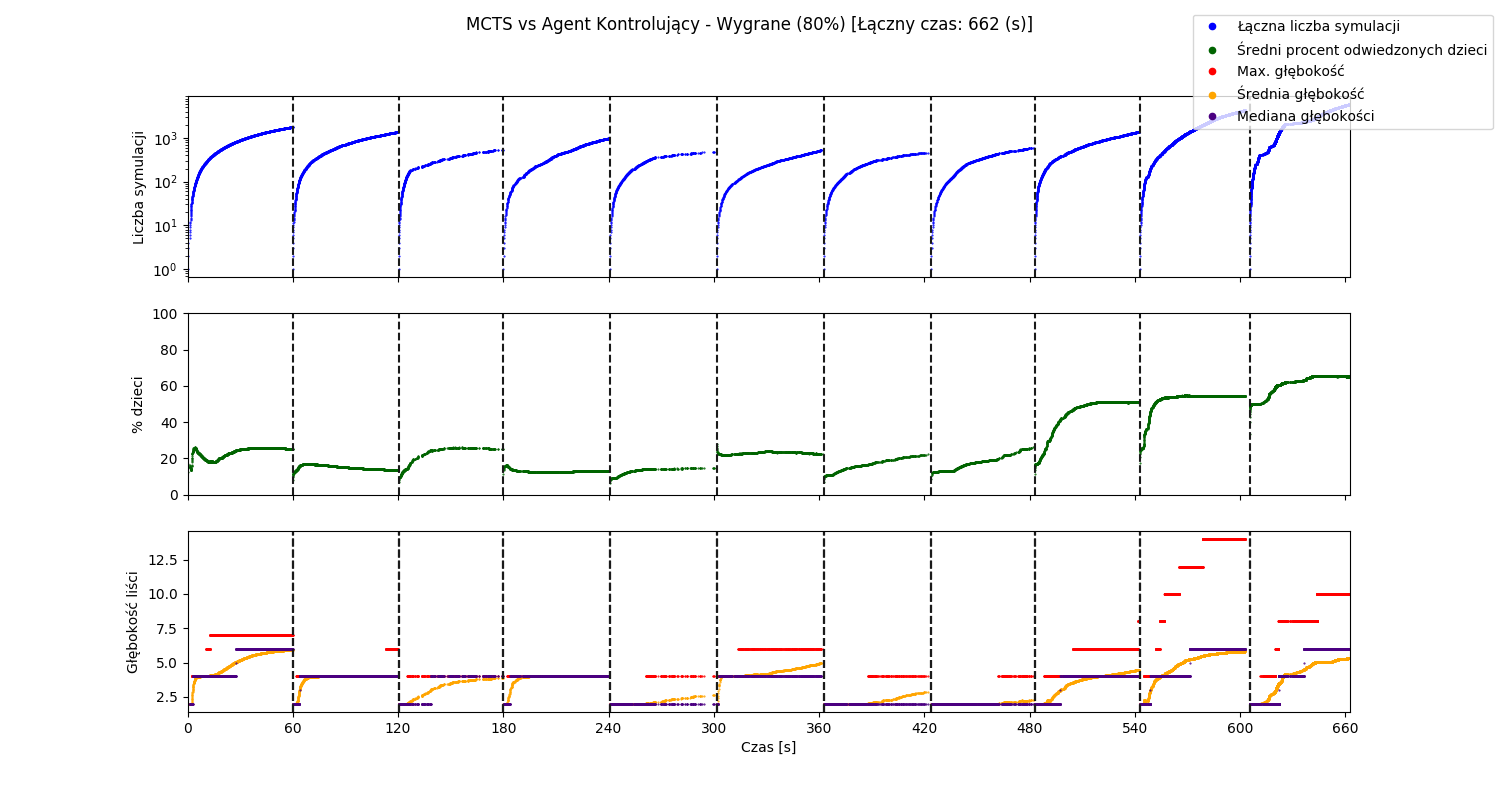
\includegraphics[width=\textwidth]{imgs/plots/MCTS_CA_WIN.png}
    \end{figure}

    \begin{figure}[H]
        \center
        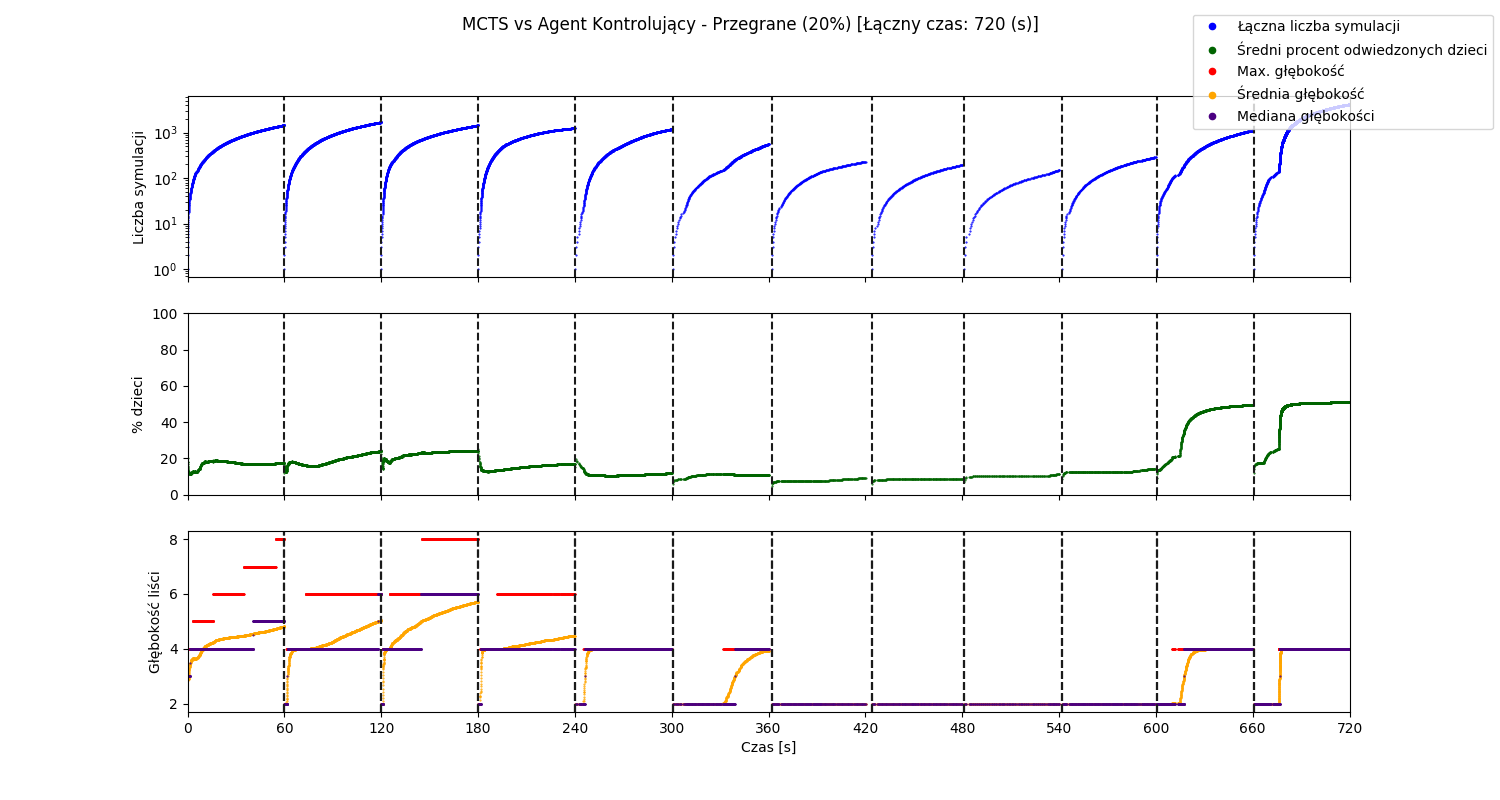
\includegraphics[width=\textwidth]{imgs/plots/MCTS_CA_LOST.png}
    \end{figure}


